\cleardoublepage
\section{\secState{R}Space Discretization - Avoidance Grid}\label{s:AvoidanceGrid}

\paragraph{Operation Space:} The \emph{Operation Space} is a space where UAS can effectively surveillance its surroundings, and it has the capability to act.

\paragraph{A Motivation for Discretization:} The UAS surroundings needs to be represented in an \emph{avoidance-friendly manner}, following principles matters:

\begin{enumerate}
	\item \emph{Discrete representation} - the space around UAS should be segmented into finite and exclusive portions which are considered as one point of the grid. This enables fast situation assessment. 
	
	\item \emph{Threat proximity} - a threat in any form is getting more important with decreasing distance to UAS.
	
	\item \emph{LiDAR swipe density} - one LiDAR swipe scans many points; the grid needs to be customized to swipe characteristics.
\end{enumerate}


The \emph{Main Sensor} is \emph{LiDAR} (problems \ref{eq:basicProblemDefinition}.-\ref{pro:rulesOfTheAir}).  The \emph{effective occupancy computation} needs to be done for all problems; the inspiration is taken from \cite{homm2010efficient}.  The \emph{effective occupancy computation} is done in \emph{LiDAR} scan  portioned into \emph{polar coordinates grid}. The \emph{operation space} is abstracted as a \emph{grid} where \emph{space portions} are representing the points in the grid.

\begin{note}
	Each member of the grid is a cell, represented as a point with shared properties, like threat level, visibility.
\end{note}

The \emph{Discrete Situation Evaluation} is executed for a \emph{UAS} local coordinate frame in fixed \emph{time}.  The goal is to enable \emph{fast discrete situation assessment}. 


\paragraph{LiDAR Swipe:} The \emph{point} scanned by \emph{LiDAR}, where the \emph{UAS position} is center of the \emph{local coordinate frame}, and \emph{UAS heading is defining the main axes} is given as:

\begin{equation}\label{eq:LiDARPoint}
    point = [distance,horizontal^\circ,vertical^\circ].
\end{equation}

\begin{note}
    For polar/Euclidean transformations and local/global coordinate frames refer to background theory (app. \ref{sec:complementsOfAlgebra}). 
    
    The \emph{right side} of UAS $horizontal^\circ$ $\in$ $]-\pi,0[$, the \emph{left-side} of UAS $horizontal^\circ$ $\in$ $[0,\pi]$, the \emph{down-side} of UAS $vertical^\circ$ $\in$ $]-\pi,0[$, the \emph{top side} of UAS $vertical^\circ$ $\in$ $[0,\pi]$
\end{note}

\paragraph{LiDAR Swipe Portioning:} The \emph{polar coordinate space} can be portioned into distinctive cells, which contains the portion space. This cell then represents one point in the grid.

The \emph{reason} for this swipe portioning is \emph{LiDAR} scanning density\footnote{Example rotary LiDAR Velodyne VL-16 specs: \url{https://www.cadden.fr/wp-content/uploads/2017/02/Velodyne_VLP-16-Puck.pdf}}, which is extremely dense. The \emph{threat} state in the cell can be assessed with linear complexity. 

The \emph{polar $\to$ euclidean} coordinate frame transformation is not amenable  for LiDAR swipe. The \emph{threat} assessment based on \emph{LiDAR swipe} in \emph{planar space portions} has minimal complexity, and it is cost effective. \cite{gupta2010comparative}.


\paragraph{Cell:} To discretize operational space into a grid of points there is a need to define cell space, which bounds the portion of the \emph{local planar coordinate frame}. The point (eq. \ref{eq:LiDARPoint}) is defined by distance, horizontal$^\circ$ offset angle, and vertical$^\circ$ offset angle. The cell is a closed compact set of such points. The boundary can be defined like follow: 

\begin{definition}{Cell}\label{def:cell}
	
    \noindent The \emph{cell} bounds a portion of space in UAS local polar coordinate frame, defined by boundary ranges:
    \begin{enumerate}
        
        \item \emph{Distance Range} -  starts and ends: $distance_{start}$ $<$ $distance_{end}$ $in$ $\R^+$.
        
        \item \emph{Horizontal Range} - starts and ends: $horizontal^\circ_{start}$ $<$ $horizontal^\circ_{end}$ $\in$ $]-\pi,\pi]$.
        
        \item \emph{Vertical Range} - starts and ends: by $vertical^\circ_{start}$ $<$ $vertical^\circ_{end}$ $\in$ $]-\pi,\pi]$.
    \end{enumerate}
    
    \noindent The \emph{space portion} belonging to the \emph{cell} is given by function as:
    
    \begin{multline}\label{eq:boundedSpaceCell}
        cell.space Portion\dots\\
            \left \{
                \begin{aligned}
                point& \in \R^3 \text{ where}:\\
                    &\left(\begin{aligned}
                        cell.distance_{start} &<& point.distance &\le& cell.distance_{end},\\
                        cell.horizontal^\circ_{start} &<& point.horizontal^\circ &\le&  cell.horizontal^\circ_{end},\\
                        cell.vertical^\circ_{start} &<& point.vertical^\circ &\le& cell.vertical^\circ_{end}\\
                    \end{aligned}\right)
                \end{aligned}
            \right\}
    \end{multline}
    
    \noindent To evaluate a \emph{static obstacle threat}, it is necessary to know how many LiDAR hits landed in the cell space portion. For one \emph{LiDAR Scan} the \emph{hits set} is given a \emph{set} of \emph{all points} which lands into cell space portion:
    \begin{equation}\label{eq:LidarHitsCell}
        cell. LiDAR Hits = \left\{point \in Lidar Scan:  point \in cell. space Portion\right\}    
    \end{equation}
    
    %\noindent The \emph{passing hits} for cell are hits which are going through the cell (passing), but it lands in distance greater than $cell.distance_{end}$, defined as:
%    \begin{multline}\label{eq:passingHitsCell}
%        Passing Hits(cell)=
%        \dots\\
%            \left \{
%                \begin{aligned}
%                point& \in Lidar Scan \text{ where}:\\
%                    &\left(\begin{aligned}
%                        cell.distance_{end}&<& point.distance &&,\\
%                        cell.horizontal^\circ_{start} &<& point.horizontal^\circ &\le&  %cell.horizontal^\circ_{end},\\
%                        cell.vertical^\circ_{start} &<& point.vertical^\circ &\le& %cell.vertical^\circ_{end}\\
%                    \end{aligned}\right)
%                \end{aligned}
%            \right\}
%    \end{multline}
\end{definition}

\begin{note}
    The \emph{cell} space portion volume is increasing with the distance. This satisfies the requirement for threat-distance importance.  The cell is considered as a point of the grid with common properties abstraction valid for all cell space portion.    
\end{note}

\paragraph{Effective Operation Space:} The goal is to determine which of the operation space is going to be considered in our avoidance grid.  The effective operation space determination according to \cite{zaiane2002clustering} is influenced by the following factors:

\begin{enumerate}
        \item \emph{Sensors ranges} -  there is no reason to assess the situation over effective \emph{sensor range}.
        
        \item \emph{Information sources} impact - there is no real impact on \emph{effective space boundary}, the information search and intersection algorithms are only of the importance.
        
        \item \emph{UAS maneuverability} - the space where UAS can maneuver, bounded by space-time (reach set boundary). 
        
        \item \emph{Computation power} - the situation evaluation and threat assessment capabilities of the onboard computer.
        
        \item \emph{Airworthiness requirements} - the \emph{regulations} can impose some minimal requirements on \emph{effective operation space boundary}.
\end{enumerate}

Let show an example of an \emph{effective operation space} for the UAS  (fig. \ref{fig:LidarSpaceSegmentation}).  The \emph{full LiDAR Swipe} (cyan and red lines) of \emph{UAS} (blue plane) has a \emph{shape} of the conical cylinder. 

\begin{note}
Under \emph{ideal circumstances}, the \emph{LiDAR swipe} would have a \emph{ball shape}, but in real cases the \emph{UAS body portion} where \emph{LiDAR} is mounted is unused.
\end{note}

The \emph{frontal portion} (red line) is a set of cells where \emph{UAS} can make maneuvers. According to the \emph{previous conditions}, there is no reason to consider a  space portion out of the maneuverable area. 

\begin{figure}[H]
    \centering
    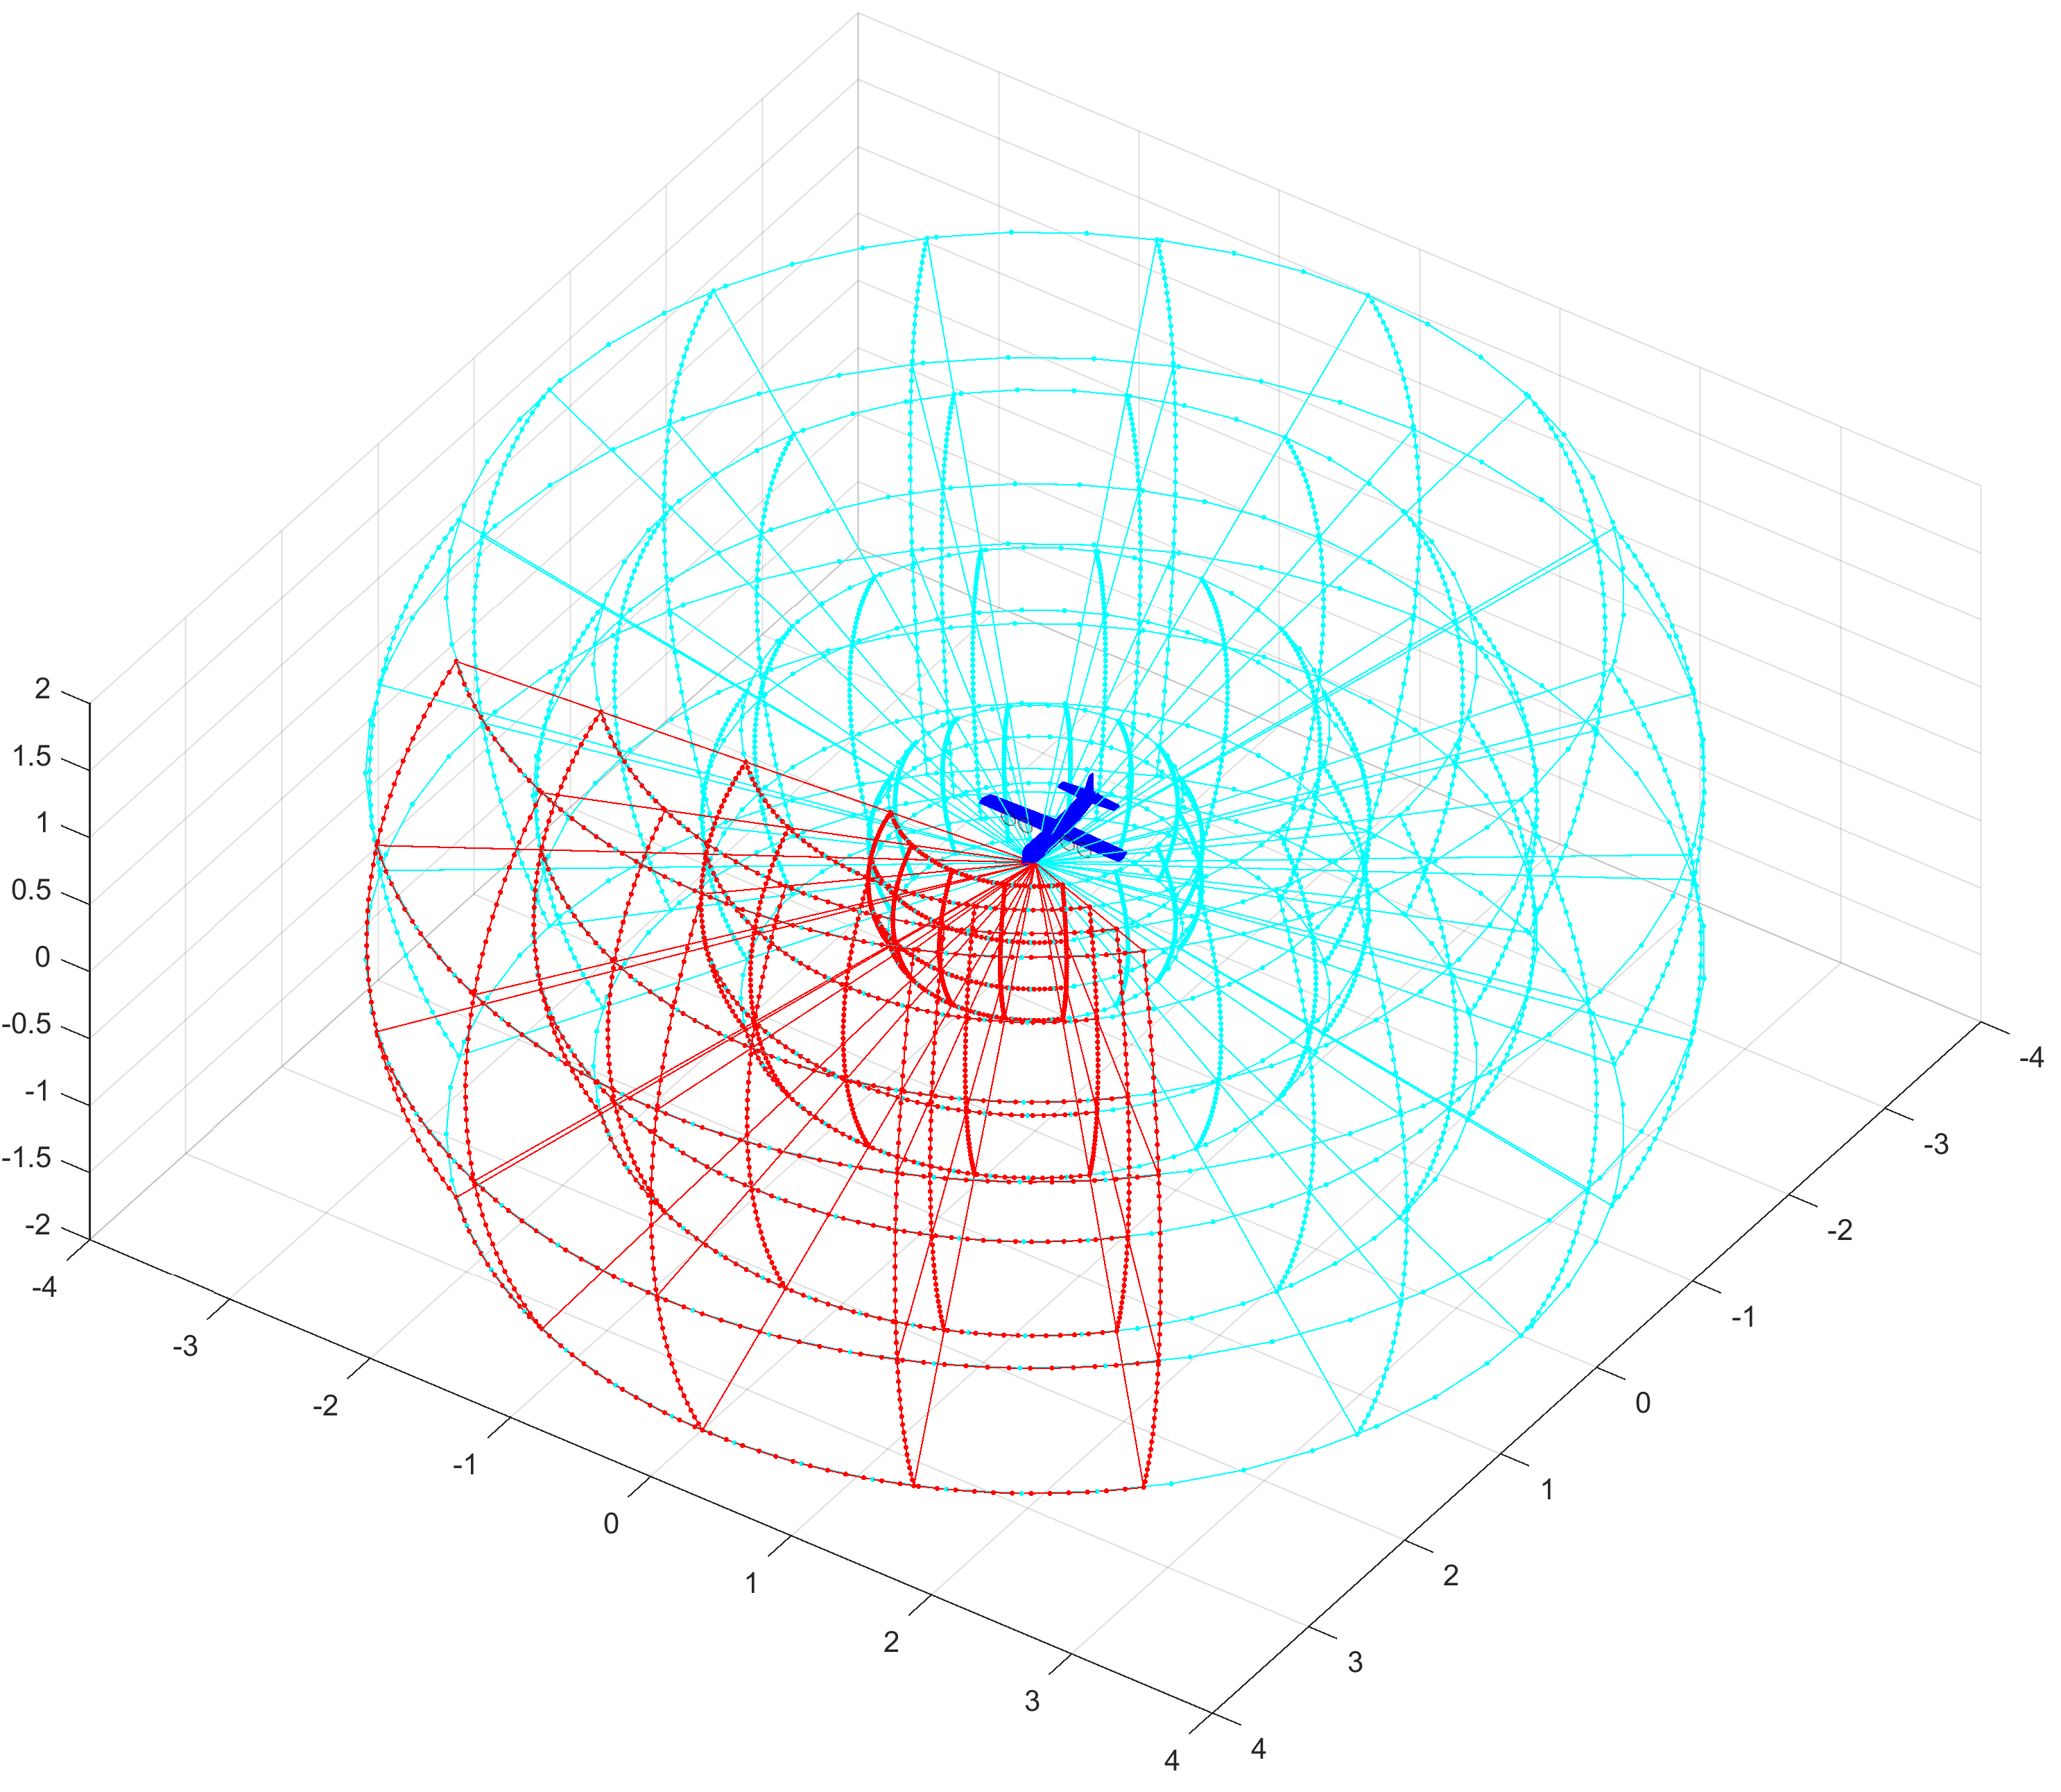
\includegraphics[width=0.80\linewidth]{\FIGDIR/TE046LiDARRasterRange} 
    \caption{Example: The \emph{LiDAR} reading portioning - cells.}
    \label{fig:LidarSpaceSegmentation}
\end{figure}

\paragraph{Avoidance Grid Definition:} The \emph{effective operation space} is going to be portioned into cells. The set of these cells is going to be called \emph{Avoidance Grid}. The idea is to split operational space into cells with even distance, horizontal angle, and vertical angle ranges. 

\begin{definition}{Avoidance Grid}\label{def:AvoidanceGrid} 


\noindent The \emph{effective space portion} (fig. \ref{fig:LidarSpaceSegmentation} red lines) given by a portion of space in UAS local polar coordinate frame, bounded by:
    \begin{enumerate}
        \item \emph{Distance Range} -  in range $distance_{start}$ $<$ $distance_{end}$ $in$ $\R^+$.
        \item \emph{Horizontal Range} - in range by $horizontal^\circ_{start}$ $<$ $horizontal^\circ_{end}$ $\in$ $]-\pi,\pi]$.
        \item \emph{Vertical Range} -in range $vertical^\circ_{start}$ $<$ $vertical^\circ_{end}$ $\in$ $]-\pi,\pi]$.
    \end{enumerate}

\noindent The goal is to separate the \emph{effective operation space} into cells (def. \ref{def:cell}). The idea is to split distance range into multiple distinctive distance ranges with count $layerCount \in \N^+$.  The ranges for \emph{distance layers} are given as follow:
\begin{equation}\label{eq:avoidanceGridCellDistanceRange}
    \begin{aligned}
        layer^i_{start} & = (i-1)\times\frac{distance_{end}-distance_{start}}{layer Count}\\
        layer^i_{end} & = i\times\frac{distance_{end}-distance_{start}}{layer Count}
    \end{aligned};\quad i\in 1\dots layer Count
\end{equation}

\noindent The same separation Layer horizontal/vertical separations defined by $horizontal Count \in \N^+$/$vertical Count \in \N^+$:

\begin{equation}\label{eq:avoidanceGridCellHorizontalRange}
    \begin{aligned}
        horizontal^j_{start} & = (j-1)\times\frac{horizontal^\circ_{end}-horizontal^\circ_{start}}{horizontal Count}\\
        horizontal^j_{end} & = j\times\frac{horizontal^\circ_{end}-horizontal^\circ_{start}}{horizontal Count}
    \end{aligned};\quad j\in 1\dots horizontal Count
\end{equation}


\begin{equation}\label{eq:avoidanceGridCellVerticalRange}
    \begin{aligned}
        vertical^k_{start} & = (k-1)\times\frac{vertical^\circ_{end}-vertical^\circ_{start}}{vertical Count}\\
        vertical^k_{end} & = k\times\frac{vertical^\circ_{end}-vertical^\circ_{start}}{vertical Count}
    \end{aligned};\quad k\in 1\dots vertical Count
\end{equation}


\noindent Then $cell_{i,j,k}$ space portion by (def. \ref{def:cell}) has the following ranges:
\begin{enumerate}
    \item \emph{Cell Distance Range} (eq. \ref{eq:avoidanceGridCellDistanceRange}) depending on layer index $i$.
    
    \item \emph{Cell Horizontal Angle Range} (eq. \ref{eq:avoidanceGridCellHorizontalRange}) depending on horizontal angle index $j$.
    
    \item \emph{Cell Vertical Angle Range} (eq. \ref{eq:avoidanceGridCellVerticalRange}) depending on vertical index $k$.
\end{enumerate}

\begin{note}
	The example of \emph{Avoidance Grid Cells} is given in (fig. \ref{fig:LidarSpaceSegmentation} red boundary).
\end{note} 

The \emph{Avoidance Grid} is the set of cells:

\begin{equation}\label{eq:avoidanceGridCellSpace}
    Avoidance Grid = \left\{
    					cell_{i,j,k}:
    					\begin{aligned}
    						& i \in 1 \dots layer Count\\
    						& j \in 1 \dots horizontal Count\\
    						& k \in 1 \dots vertical Count
    					\end{aligned} 
                     \right\}
\end{equation}

\begin{note}
	For any distinctive cells $cell_{i,j,k}$, $cell_{m,n,o}$ their \emph{space portion intersection} is empty set:
	\begin{equation}
		\forall cell_{i,j,k}, cell_{m,n,o}:
		\begin{aligned}
		    &cell_{i,j,k}\cap cell_{m,n,o} = \varnothing,
		    i \neq o \lor j \neq n \lor k \neq o
		\end{aligned}
	\end{equation}
\end{note}
\end{definition}

%\paragraph{Trajectory Intersection:} The \emph{trajectory} intersection with \emph{Avoidance Grid} is solved in context of \emph{Reach Set Approximation} (def. \ref{def:ContainedReducedReachSet}). 
%\begin{note}
%    The \emph{trajectory intersection} function does not have an impact on \emph{Reach Set Approximation}, because its done prior the flight.
%\end{note}

\paragraph{Grid Sizing Approach:} The sizing approach used in this work is outlined in (app. \ref{app:gridSizeCalculation}).


\paragraph{Cell in Avoidance Grid Properties:}\noindent For each cell $\vec{p}\in\R^3$ in the there are properties to be checked:

\begin{enumerate}
    \item \emph{Is there visibility to the cell?} - how good is an observation of the cell by Sensor Field.
    
    \item \emph{Is there threat present?} - how sure the data fusion is that there is eminent threat in the cell.
    
    \item \emph{Is the cell reachable?} - if there is any trajectory which can get UAS to that cell without too much threat along the way.
\end{enumerate}

\noindent The answers to these questions are given later in \emph{data fusion procedure} outline (tab. \ref{tab:defuzificationRatings}).
